% Run this file with pdflatex.
%
%\pdfhorigin-72bp
%\pdfvorigin6in
% Compression of stream objects, between 0 (disable) and 9.
\pdfcompresslevel=6
% Compression of non-stream objects, between 0 and 3.
\pdfobjcompresslevel=3
\documentclass{minimal}
% Otherwise the drawing moves off the page.
\usepackage[papersize={72.4bp,73.7bp},margin=2mm]{geometry}
\usepackage{tikz}
\begin{document}
% I want to have float numbers in the MediaBox:
% The pdfpagesattr does not replace the default MediaBox
%\pdfpagesattr{ /MediaBox [-0.2 -0.9 72.2 72.8] }
% This does
\pdfpageattr{ /MediaBox [-0.2 -0.9 72.2 72.8] }
\noindent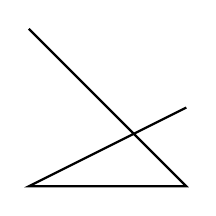
\begin{tikzpicture}
\draw[thick] (0,2) -- (2,0) -- (0,0) -- (2,1);
\end{tikzpicture}
\end{document}
%%% pict2e variant:
% \usepackage{pict2e}
% \begin{document}
% \noindent\begin{picture}(60,60)
% \thicklines\polyline(0,54)(54,0)(0,0)(54,36)
% \end{picture}
